% TikZ source for manuscript Figure 1 — CSE architecture.
% Render: pdflatex fig1_architecture.tex  (or `make figures` matplotlib fallback)
\documentclass[tikz,border=8pt]{standalone}
\usepackage{tikz}
\usetikzlibrary{arrows.meta,positioning,fit,shapes.geometric}
\begin{document}
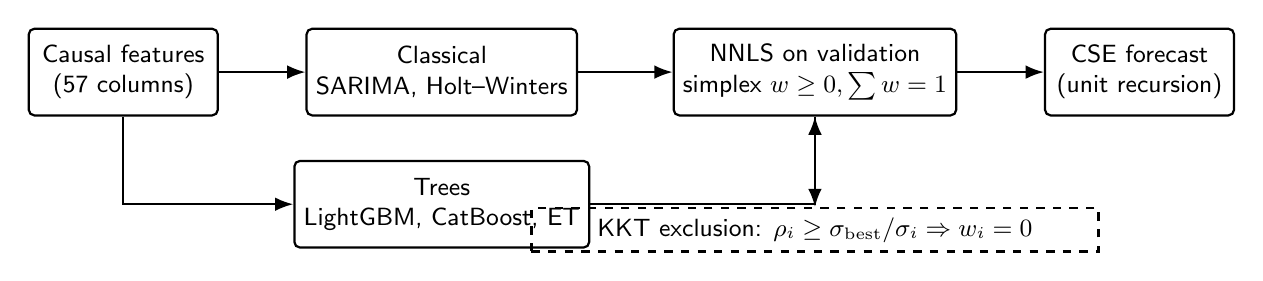
\begin{tikzpicture}[
  font=\sffamily\small,
  box/.style={draw, thick, align=center, rounded corners=2pt, minimum height=1.1cm, minimum width=2.4cm},
  arrow/.style={-{Latex}, thick}
]
\node[box] (feat) {Causal features\\(57 columns)};
\node[box, right=1.1cm of feat] (class) {Classical\\SARIMA, Holt--Winters};
\node[box, below=0.55cm of class] (tree) {Trees\\LightGBM, CatBoost, ET};
\node[box, right=1.2cm of class] (nnls) {NNLS on validation\\simplex $w\ge 0,\sum w=1$};
\node[box, right=1.1cm of nnls] (cse) {CSE forecast\\(unit recursion)};
\node[draw, thick, dashed, align=center, below=1.15cm of nnls, minimum width=7.2cm]
  (kkt) {KKT exclusion: $\rho_i \ge \sigma_{\mathrm{best}}/\sigma_i \Rightarrow w_i=0$};

\draw[arrow] (feat) -- (class);
\draw[arrow] (feat) |- (tree);
\draw[arrow] (class) -- (nnls);
\draw[arrow] (tree) -| (nnls);
\draw[arrow] (nnls) -- (cse);
\draw[arrow] (nnls) -- (kkt);
\end{tikzpicture}
\end{document}
